\chapter{Discussion ESB in Openshift}
\label{cha:esbd}
This chapter will evaluate the implemented prototype of Chapter \vref{cha:esbi}, and will show that challenges such as
\begin{itemize}
	\item managing multiple environments,
	\item managing multiple service versions,
	\item managing public API migration,
	\item managing adapters and transformers as services,
	\item and managing service security
\end{itemize}
are manageable tasks when hosting an ESB in Openshift. 

\section{Managing Multiple Environments}
\label{sec:esbd-multiple-env}
An ESB is commonly hosted on multiple environments, whereby at least one productive and one testing environment should be present. These environment where commonly a VM, which provides the runtime environment for the ESB. As the prototype shows, the environment is now represented by an Openshift Project, which can be reproduced easily via scripts as discussed in Section \vref{sec:esbi-openshift}. \\

The services hosted on the ESB are using Fuse integration Service 2.0 and its provided tooling, which ensure that the service are properly encapsulated in a container and properly managed in Openshift. Therefore, the service developers provide the necessary Openshift Templates, which has the effect that the operators have no interaction with the service artifacts and runtime environments anymore. Operator have only to manage
\begin{itemize}
	\item the Openshift Project, which hosts the services,
	\item the Openshift ConfigMaps, which hold the service non-sensitive configuration,
	\item the Openshift Secrets, which hold the sensitive service configuration,
	\item and scripts for utility such as backup/restore of service data or instance scaling.
\end{itemize} 
Listing \vref{ls:esboi-config-project-stages-prod} shows how developers reference Openshift Objects such as Openshift ConfigMaps and Openshift Secrets, which are managed by operators. 

\begin{figure}[htbp]
	\centering
	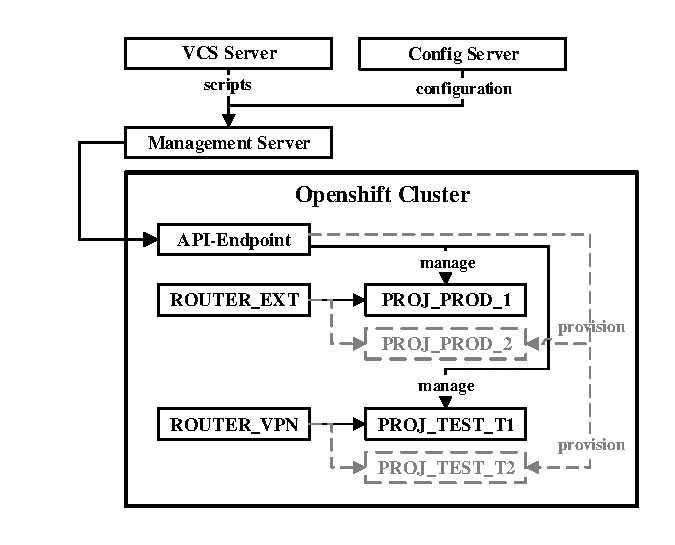
\includegraphics[scale=1]{images/esbd-multi-stage-env.pdf}
	\caption{Management and provisioning of multiple environments}
	\label{fig:esbd-multi-stage-env}
\end{figure}

Figure \vref{fig:esbd-multi-stage-env} illustrates the management and provisioning of multiple environments for an ESB, whereby the hosting environment is represented by an Openshift Project. The \mentionedtext{Management Server} pulls the scripts and Openshift Templates from a \mentionedtext{VCS Server} and the configurations from a \mentionedtext{Configuration Server}. The scripts and Openshift Templates are separated from the configurations, which are actually providing the data for the scripts and Openshift Template-Parameters. With such an approach, the infrastructure becomes reproducible, versioned, and therefore consistent, and disposable. These characteristics are also principles of IaC, which have already been discussed in Chapter \vref{cha:iac}. \\

The schema of Figure \vref{fig:esbd-multi-stage-env} is similar to the Figure \vref{fig:reproduce-infrastructure}, which illustrated how a system can be reproduced with parametrized templates and an IaC tool. The Openshift CLI provides functionality to manage Openshift Objects, which is what needs to be done when providing an environment in form of an Openshift Project, therefore the Openshift CLI acts as an IaC tool. 



%fig:reproduce-infrastructure

\section{Managing Multiple Service Versions}
\label{sec:esbd-multi-version-service}

\section{Managing Migration of Public API}
\label{sec:esbd-multi-stage-env}

\section{Managing Adapters and Transformers as Services}
\label{sec:esbd-adap-trans-service}

\section{Managing Service Security}
\label{sec:esbd-service-security}

\section{Further Work}
\label{sec:esbd-furhter-work}